\documentclass[12pt,letterpaper]{exam}
\usepackage[lmargin=1in,rmargin=1in,tmargin=1in,bmargin=1in]{geometry}
\usepackage{../style/exams}

% -------------------
% Course & Exam Information
% -------------------
\newcommand{\course}{MATH 122: Exam 3}
\newcommand{\term}{Fall --- 2024}
\newcommand{\examdate}{11/21/2024}
\newcommand{\timelimit}{75 Minutes}

\setbool{hideans}{false} % Student: True; Instructor: False

% -------------------
% Content
% -------------------
\begin{document}

\examtitle
\instructions{Write your name on the appropriate line on the exam cover sheet. This exam contains \numpages\ pages (including this cover page) and \numquestions\ questions. Check that you have every page of the exam. Answer the questions in the spaces provided on the question sheets. Be sure to answer every part of each question and show all your work. If you run out of room for an answer, continue on the back of the page --- being sure to indicate the problem number.} 
\scores
\bottomline
\newpage


% -------------------
% Questions
% -------------------
\begin{questions}

% Question 1
\newpage
\question[15] Consider the plot of a function $f(x)$ given below.
	\[
	\fbox{
	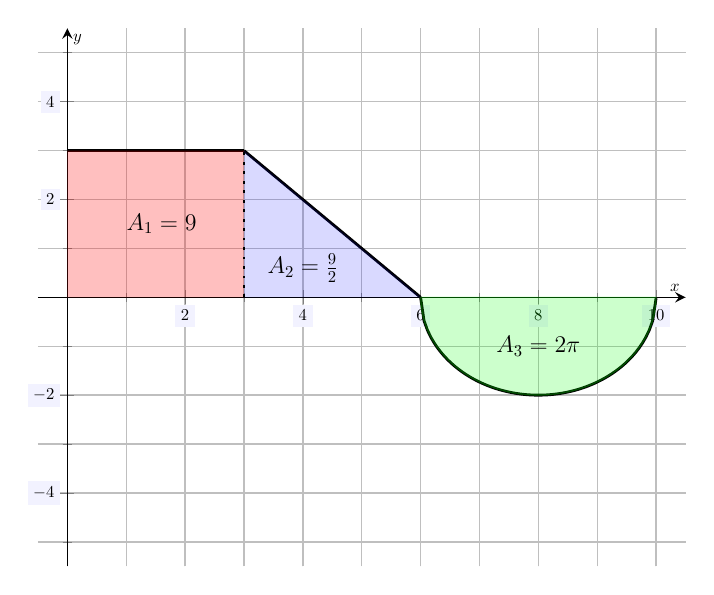
\begin{tikzpicture}[scale=1.2,every node/.style={scale=0.5}]
	\begin{axis}[
	grid=both,
	axis lines=middle,
	ticklabel style={fill=blue!5!white},
	xmin= -0.5, xmax=10.5,
	ymin= -5.5, ymax=5.5,
	xtick={-2,0,...,10},
	ytick={-6,-4,...,6},
	minor tick = {-10,-9,...,10},
	xlabel=\(x\),ylabel=\(y\),
	]
	\addplot[line width= 0.03cm,samples=5,domain= 0:3] ({x},{3});
	\addplot[line width= 0.03cm,samples=5,domain= 3:6] ({x},{6 - x});
	\addplot[line width= 0.03cm,samples=70,domain= 6:10] ({x},{-sqrt(4 - (x - 8)^2)});
	\node at (1,7.2) {$f(x)$};
	
	\draw[draw=none,fill=red,opacity=0.25] (0,0) -- (3,0) -- (3,3) -- (0,3) -- (0,0);
	\draw[draw=none,fill=blue,opacity=0.15] (3,0) -- (6,0) -- (3,3) -- (3,0);
	\draw[green,fill=green,opacity=0.2] (6,0) arc (180:360:2) -- (6,0);
	\draw[line width=0.03cm,dotted] (3,0) -- (3,3);
	\node at (1.6,1.5) {\Large$A_1= 9$};
	\node at (4,0.6) {\Large$A_2= \frac{9}{2}$};
	\node at (8,-1) {\Large$A_3= 2\pi$};
	\end{axis}
	\end{tikzpicture}
	}
	\]
Using the above plot, compute the following: \par\vspace{0.3cm}
	\begin{enumerate}[(a)]
	\item $\displaystyle\int_0^3 f(x) \;dx= A_1= bh= 3(3)= 9$ \vfill
	
	\item $\displaystyle\int_6^{10} f(x) \;dx= -A_3= -\dfrac{1}{2}\, \pi r^2= -\dfrac{1}{2} \cdot \pi (2^2)= -\dfrac{1}{2} \cdot 4\pi= -2\pi \approx -6.28319$ \vfill
	
	\item $\displaystyle\int_0^{10} f(x) \;dx= A_1 + A_2 + (-A_3)= 9 + \dfrac{9}{2} - 2\pi= \dfrac{27}{2} - 2\pi \approx 7.21681$ \vfill
	
	\item $\displaystyle\int_5^5 f(x) \;dx= 0$ \vfill
	
	\item The area between $f(x)$ and the $x$-axis. 
		\[
		A_1 + A_2 + A_3= 9 + \dfrac{9}{2} + 2\pi= \dfrac{27}{2} + 2\pi \approx 19.7832
		\]
	\end{enumerate}



% Question 2
\newpage
\question[15] A jet plane is descending for a landing. The velocity in mph at a time $t$~minutes from the start of its descent, $v(t)$, is given in the table below.
	\begin{table}[!ht]
	\centering
	\begin{tabular}{|l||c|c|c|c|c|c|c|} \hline
	Time, $t$ & 0 & 5 & 10 & 15 & 20 \\ \hline
	Velocity, $v(t)$ & 550 & 520 & 500 & 490 & 410 \\ \hline
	\end{tabular}
	\end{table}

\begin{enumerate}[(a)]
\item Using the table above and a right-hand sum, approximate $\displaystyle\int_0^{20} v(t) \;dt$ as accurately as possible. \pspace

	{\itshape We can create a rough sketch of the right-hand sum:
	\[
	\fbox{
	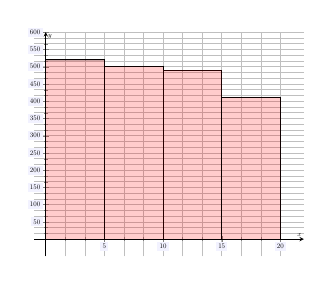
\begin{tikzpicture}[scale=0.5,every node/.style={scale=0.5}]
	\begin{axis}[
	grid=both,
	axis lines=middle,
	ticklabel style={fill=blue!5!white},
	xmin= -1, xmax=22,
	ymin= -50, ymax=600,
	xtick={0,5,...,20},
	ytick={0,50,...,600},
	minor y tick num= 2,
	minor x tick num=2,
	xlabel=\(x\),ylabel=\(y\),
	]
	\draw[line width=0.02cm] (0,0) -- (5,0) --(5,520) -- (0,520) -- (0,0);
	\draw[fill=red,opacity=0.20] (0,0) -- (5,0) --(5,520) -- (0,520) -- (0,0);
	\draw[line width=0.02cm] (5,0) -- (10,0) -- (10,500) -- (5,500) -- (5,0);
	\draw[fill=red,opacity=0.20] (5,0) -- (10,0) -- (10,500) -- (5,500) -- (5,0);
	\draw[line width=0.02cm] (10,0) -- (15,0) -- (15,490) -- (10,490) -- (10,0);
	\draw[fill=red,opacity=0.20] (10,0) -- (15,0) -- (15,490) -- (10,490) -- (10,0);
	\draw[line width=0.02cm] (15,0) -- (20,0) -- (20,410) -- (15,410) -- (15,0);
	\draw[fill=red,opacity=0.20] (15,0) -- (20,0) -- (20,410) -- (15,410) -- (15,0);
	\end{axis}
	\end{tikzpicture}
	}
	\] 
	Computing the total area of these rectangles, we have\dots
		\[
		\int_0^{20} v(t) \;dt \approx 5(520) + 5(500) + 5(490) + 5(410)= 2600 + 2500 + 2450 + 2050= 9600
		\]
	} \par\vspace{0.7cm}

\item What does your value in (a) represent? \pspace

	{\itshape We know that $v(t)$ has units of miles per hour. But then $\int v(t) \;dt$ has units of $\text{mph} \cdot \text{hr}= \text{miles}$. We know the integral of a rate over an interval gives the net change of that function over that interval. Therefore, $\displaystyle\int_0^{20} v(t) \;dt \approx 9600$ represents that the plane has approximately traveled an additional 9,600~miles.} \par\vspace{1.1cm}
	
\item Based on the table is your approximation in (a) likely an under- or over-estimate? \pspace
	
	{\itshape Because the speed seems to be consistently decreasing, we make the assumption the speed is only decreasing. But then using the right-endpoint would use the lowest possible speed on each time interval. Therefore, we get the smallest possible area, i.e. the smallest possible increase to the net distance traveled. Therefore, the approximation in (a) is likely an underestimate.}
\end{enumerate}



% Question 3
\newpage
\question Showing all your work, compute the following: \par\vspace{0.3cm}
	\begin{parts}
	\part[5] $\displaystyle\int (\sqrt{x} + e^x) \;dx$ \vfill
	
		\[
		\int (\sqrt{x} + e^x) \;dx= \int \left( x^{1/2} + e^x \right) \;dx= \dfrac{x^{3/2}}{3/2} + e^x + C= \dfrac{2}{3}\, x^{3/2} + e^x + C
		\] \vfill
	
	\part[5] $\displaystyle\int_{-1}^1 \left( x^3 - 6x^2 \right) \;dx$ \vfill
	
		\[
		\hspace{-2.5cm} \int_{-1}^1 \left( x^3 - 6x^2 \right) \;dx= \dfrac{x^4}{4} - \dfrac{6x^3}{3} \bigg|_{-1}^1= \dfrac{x^4}{4} - 2x^3 \bigg|_{-1}^1= \left( \dfrac{1}{4} - 2(1) \right) - \left( \dfrac{1}{4} - 2(-1) \right)= -\dfrac{7}{4} - \dfrac{9}{4}= -\dfrac{16}{4}= -4
		\] \vfill
	
	\part[5] $\displaystyle\int \left( 5^x - \dfrac{2}{x} \right)\;dx$ \vfill
	
		\[
		\int \left( 5^x - \dfrac{2}{x} \right)\;dx= \dfrac{5^x}{\ln 5} - 2 \ln |x| + C
		\] \vfill
	\end{parts}



% Question 4
\newpage
\question[10] Showing all your work, use a left-hand sum with three evenly spaced rectangles to approximate the following:
	\[
	\int_1^{13} \left( x \ln x - 1 \right) \;dx
	\] \pspace

{\itshape \tsol Because the integral begins at $a= 1$, ends at $b= 13$, and we will use $n= 3$ evenly spaced rectangles, each rectangle must have width\dots
	\[
	\Delta x= \dfrac{b - a}{n}= \dfrac{13 - 1}{3}= \dfrac{12}{3}= 4
	\]
We can even create a sketch to help visualize the integral---the accuracy of the actual function curve is not important:
	\[
	\fbox{
	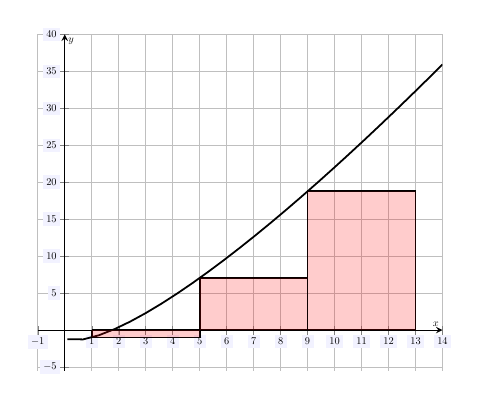
\begin{tikzpicture}[scale=0.75,every node/.style={scale=0.5}]
	\begin{axis}[
	grid=both,
	axis lines=middle,
	ticklabel style={fill=blue!5!white},
	xmin= -1, xmax=14,
	ymin= -5.5, ymax=40,
	xtick={-1,0,...,14},
	ytick={-5,0,5,...,40},
	xlabel=\(x\),ylabel=\(y\),
	]
	\addplot[line width=0.03cm,domain=0.1:14] ({x},{x*ln(x) - 1});
	\draw[line width=0.03cm] (1,0) -- (5,0) -- (5,-1) -- (1,-1) -- (1,0);
	\draw[fill=red,opacity=0.20] (1,0) -- (5,0) -- (5,-1) -- (1,-1) -- (1,0);
	\draw[line width=0.03cm] (5,0) -- (9,0) -- (9,7.05) -- (5,7.05) -- (5,0);
	\draw[fill=red,opacity=0.20] (5,0) -- (9,0) -- (9,7.05) -- (5,7.05) -- (5,0);
	\draw[line width=0.03cm] (9,0) -- (13,0) -- (13,18.78) -- (9,18.78) -- (9,0);
	\draw[fill=red,opacity=0.20] (9,0) -- (13,0) -- (13,18.78) -- (9,18.78) -- (9,0);
	\end{axis}
	\end{tikzpicture}
	}
	\] 
Letting $f(x)= x \ln x - 1$, the left-hand sum is\dots
	\[
	\begin{aligned}
	\int_1^{13} \left( x \ln x - 1 \right) \;dx &\approx 4 f(1) + 4 f(5) + 4 f(9) \\[0.3cm]
	&\phantom{\approx}= 4 (1 \ln(1) - 1) + 4 (5 \ln(5) - 1) + 4 (9 \ln(9) - 1) \\[0.3cm]
	&\phantom{\approx}= 4(-1) +  4(7.04719) + 4(18.775) \\[0.3cm]
	&\phantom{\approx}= -4 + 28.1888 + 75.1 \\[0.3cm]
	&\phantom{\approx}= 99.2888
	\end{aligned}
	\]

\vfill Note. The actual value of the given integral is approximately $\displaystyle \int_1^{13} (x \ln x - 1) \;dx \approx 162.738$. The approximation is above has only a 38.99\% error using only three rectangles. 
}



% Question 5
\newpage
\question Showing all your work, compute the following: \par\vspace{0.3cm}
	\begin{parts}
	\part[5] $\displaystyle\int \dfrac{x^3 - 5x^2 + 6}{x^2} \;dx$ \vfill
	
		\[
		\hspace{-1.5cm} \int \dfrac{x^3 - 5x^2 + 6}{x^2} \;dx= \int \left( \dfrac{x^3}{x^2} - \dfrac{5x^2}{x^2} + \dfrac{6}{x^2} \right) \;dx= \int \left( x - 5 + 6x^{-2} \right) \;dx= \dfrac{1}{2}\, x^2 - 5x - 6x^{-1} + C
		\] \vfill
	
	\part[5] $\displaystyle\int (x^4 + 3)^2 \;dx$ \vfill
	
		\[
		\int (x^4 + 3)^2 \;dx= \int (x^4 + 3)(x^4 + 3) \;dx= \int (x^8 + 6x^4 + 9) \;dx= \dfrac{1}{9}\, x^9 + \dfrac{6}{5}\,x^5 + 9x + C
		\] \vfill
	\end{parts}



% Question 6
\newpage
\question Showing all your work, use $u$-substitution to compute the following: \par\vspace{0.3cm}
	\begin{parts}
	\part[5] $\displaystyle\int x \sqrt{3x^2 + 5} \;dx$ \pspace
	
	{\itshape We have\dots
		\[
		\begin{aligned}
		u= 3x^2 + 5
		\end{aligned}
		\qquad \qquad \qquad
		\begin{aligned}
		du= 6x \;dx \\[0.1cm]
		dx= \dfrac{1}{6x}\,du
		\end{aligned}
		\]
	Therefore, we have\dots
		\[
		\begin{aligned}
		\int x \sqrt{3x^2 + 5} \;dx&= \int x \sqrt{u} \cdot \dfrac{1}{6x}\;du \\
		&= \int \dfrac{1}{6}\, \sqrt{u}\;du \\
		&= \dfrac{1}{6} \int u^{1/2} \;du \\
		&= \dfrac{1}{6} \cdot \dfrac{2}{3}\,u^{3/2} + C \\
		&= \dfrac{1}{9}\, u^{3/2} + C \\
		&= \dfrac{1}{9} \left( 3x^2 + 5 \right)^{3/2} + C
		\end{aligned}
		\]
	} \vfill
	
	\part[5] $\displaystyle\int_0^4 (5 - 2x)^3 \;dx$ \pspace
	
	{\itshape We have\dots
		\[
		\begin{gathered}
		u= 5 - 2x \\[0.5cm]
		du= -2 \;dx \\
		dx= -\dfrac{1}{2}\,du \\[0.5cm]
		\end{gathered}
		\qquad \qquad \qquad
		\begin{gathered}
		x=0 \colon u= 5 - 2(0)= 5 - 0= 5 \\[0.3cm]
		x=4 \colon u= 5 - 2(4)= 5 - 8= -3
		\end{gathered}
		\]
	Therefore, we have\dots
		\[
		\int_0^4 (5 - 2x)^3 \;dx= \int_5^{-3} u^3 \cdot -\dfrac{1}{2} \;du= -\dfrac{1}{2} \int_5^{-3} u^3 \;du= -\dfrac{1}{2} \cdot \dfrac{u^4}{4} \bigg|_5^{-3}= -\dfrac{1}{8}\, u^4 \bigg|_5^{-3}
		\]
	But then, we have\dots
		\[
		\int_0^4 (5 - 2x)^3 \;dx== -\dfrac{1}{8} \left( (-3)^4 - 5^4 \right)= -\dfrac{1}{8} \left( 81 - 625 \right)= -\dfrac{1}{8} \cdot -544= 68
		\]
	} \vfill
	\end{parts}



% Question 7
\newpage
\question[15] The marginal cost of producing $q$ dill pickle scented candles is given by $C'(q)= 1.5 + \dfrac{100}{2q + 1}$. The total cost to produce 6,000 candles is \$34,500. 
	\begin{enumerate}[(a)]
	\item Find the cost function, $C(q)$.
	\item What are the fixed costs?
	\item Find the cost to produce 20,000 candles?
	\end{enumerate} \pspace

{\itshape
\begin{enumerate}[(a)]
\item We know that up to a constant, the total cost function is given by $\displaystyle C(q)= \int C(q) \;dq$. We have\dots
	\[
	C(q)= \int C'(q) \;dq= \int \left(1.5 + \dfrac{100}{2q + 1} \right) dq= \int 1.5 \;dq + \int \dfrac{100}{2q + 1}\; dq
	\]
We know that $\displaystyle \int 1.5 \;dq= 1.5q$. For the second integral, we use $u$-substitution: choose $u= 2q + 1$, so that $du= 2\;dq$. But then $dq= \frac{1}{2}\,du$. But then\dots
	\[
	\int \dfrac{100}{2q + 1} \;dq= \int \dfrac{100}{u} \cdot \dfrac{1}{2} \;du= \int \dfrac{50}{q} \;dq= 50 \ln|u|= 50 \ln|2q + 1|
	\]
Therefore, we have\dots
	\[
	C(q)= \int C'(q) \;dq= 1.5q + 50 \ln|2q + 1| + K
	\]
where $K$ is a constant. But we know that 6,000 candles has a total production cost of \#34,500, i.e. $C(6000)= 34500$. Therefore, we have\dots
	\[
	\begin{gathered}
	C(6000)= 34500 \\
	1.5(6000) + 50 \ln|2(6000) + 1| + K= 34500 \\
	9000 + 50 \ln(12001) + K= 34500 \\
	9000 + 469.64 + K= 34500 \\
	9469.64 + K= 34500 \\
	K= 25030.36
	\end{gathered}
	\]
Therefore, we know\dots
	\[
	C(q)= 1.5q + 50 \ln|2q + 1| + 25030.36
	\]

\item We know the fixed costs are $C(0)$. But then\dots
	\[
	\text{Fixed Costs}= C(0)= 1.5(0) + 50 \ln(1) + 25030.36= \$25,\!030.36 
	\]

\item The cost to produce 20,000 candles is\dots
	\[
	C(20000)= 1.5(20000) + 50 \ln|40001| + 25030.36= \$55,\!560.19
	\]
\end{enumerate}
}



% Question 8
\newpage
\question[10] A fresh brewed, decaf venti cup of coffee with 3 squirts of vanilla, 8 pumps of caramel, 5 sugars, and almond milk is at 195$^\circ$F. The rate of change in temperature of the coffee, measured in degrees Fahrenheit per minute, $t$ minutes from now is given by $r(t)= -15 e^{-0.25t}$. Estimate the coffee's temperature after 30~minutes. Be sure to show all your work. \pspace

{\itshape \tsol We know that\dots
	\[
	\text{Current Temperature}= \text{Initial Temperature} + \text{Change in Temperature}
	\]
We know the net change in the temperature of the coffee can be computed using the integral. Using the fact that $\displaystyle \int e^{kt} \;dt= \frac{1}{k}\, e^{kt} + C$, we have\dots
	\[
	\begin{aligned}
	\text{Change in Temperature}&= \int_0^{30} r(t) \;dt \\[0.3cm]
	&= \int_0^{30} -15 e^{-0.25t} \;dt \\[0.3cm]
	&= -15 \int_0^{30} e^{-0.25t} \;dt \\[0.3cm]
	&= -15 \cdot \dfrac{1}{-0.25}\, e^{-0.25t} \bigg|_0^{30} \\[0.3cm]
	&= 60 \cdot e^{-0.25} \bigg|_0^{30} \\[0.3cm]
	&= 60 \cdot \left(e^{-0.25 \cdot 30} - e^{-0.25 \cdot 0} \right) \\[0.3cm]
	&= 60 \cdot \left(e^{-7.5} - e^{0} \right) \\[0.3cm]
	&= 60 \cdot \left(e^{-7.5} - e^{0} \right) \\[0.3cm]
	&= 60 \cdot (0.000553084 - 1) \\[0.3cm]
	&= 60 \cdot --0.999446916 \\[0.3cm]
	&= -59.96681496 \approx -59.97
	\end{aligned}
	\]
Therefore, we have\dots
	\[
	\begin{aligned}
	\text{Current Temperature}&= \text{Initial Temperature} + \text{Change in Temperature} \\[0.3cm]
	&= 195^\circ \text{\normalfont F} - 59.97^\circ \text{\normalfont F} \\[0.3cm]
	&= 135.03^\circ \text{\normalfont F}
	\end{aligned}
	\]
}

\end{questions}
\end{document}